% 2011 年辽宁卷理科第 8 题：四棱锥 S-ABCD，底面正方形，SD⊥底面。
% 来源 PDF：普通高考/2011/2011辽宁理.pdf，SHA-256 1fe81a3887c7782547f2dc987a468a7092be184781a1190af911ebb93a28e88e。
% 原页：第 1 页第 2 栏上部，书页码 681。示意。
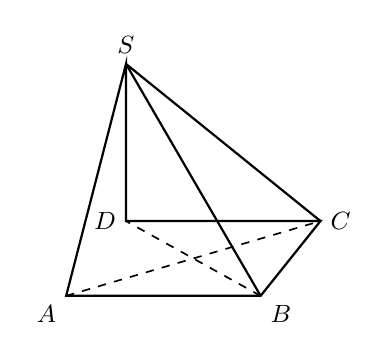
\begin{tikzpicture}[>=stealth, semithick, font=\small, scale=0.95]
  \coordinate (A) at (0,0);
  \coordinate (B) at (2.6,0);
  \coordinate (C) at (3.4,1.0);
  \coordinate (D) at (0.8,1.0);
  \coordinate (S) at (0.8,3.1);
  \draw[thick] (S)--(A)--(B)--(C)--(D)--cycle;
  \draw[thick] (S)--(B) (S)--(C);
  \draw[dashed] (S)--(D) (A)--(C) (B)--(D);
  \node[above] at (S) {$S$};
  \node[below left] at (A) {$A$};
  \node[below right] at (B) {$B$};
  \node[right] at (C) {$C$};
  \node[left] at (D) {$D$};
\end{tikzpicture}
